\documentclass[a4paper,12pt,openright, oneside]{book}
\usepackage{graphicx} % Required for inserting images
\usepackage{amsmath}
\usepackage{amssymb}
\usepackage{algorithm}
\usepackage{fancyhdr}
\usepackage{algpseudocode}
\usepackage{tcolorbox}
\usepackage{appendix}
\usepackage{accents}
% \usepackage{mathptmx}
\usepackage{url}
\usepackage[
]{todonotes}

\tcbuselibrary{minted,breakable,xparse,skins}
 \renewcommand\bibname{Viri in literatura}
  
\renewenvironment{abstract}
 {\par\noindent \hfill \textbf{Izvleček}  \hfill\ \ignorespaces \\}
 {\par\medskip \medskip}

%\addtolength{\marginparwidth}{-20pt} % robovi za tisk
%\addtolength{\oddsidemargin}{40pt}
%\addtolength{\evensidemargin}{-40pt}

\renewcommand{\chaptername}{Poglavje}
\renewcommand{\baselinestretch}{1.3} % ustrezen razmik med vrsticami
\setlength{\headheight}{15pt}        % potreben prostor na vrhu
\renewcommand{\chaptermark}[1]%
{\markboth{\MakeUppercase{\thechapter.\ #1}}{}} \renewcommand{\sectionmark}[1]%
{\markright{\MakeUppercase{\thesection.\ #1}}} \renewcommand{\headrulewidth}{0.5pt} \renewcommand{\footrulewidth}{0pt}
\fancyhf{}
\fancyhead[LE,RO]{\sl \thepage} 
%\fancyhead[LO]{\sl \rightmark} \fancyhead[RE]{\sl \leftmark}
\fancyhead[RE]{\sc \tauthor}              % dodal Solina
\fancyhead[LO]{\sc Seminarska naloga}     % dodal Solina

\renewcommand\appendixname{Priloga}
\renewcommand\appendixtocname{Priloga}

\newcommand{\BibLaTeX}{{\sc Bib}\LaTeX}
\newcommand{\BibTeX}{{\sc Bib}\TeX}

%%%%%%%%%%%%%%%%%%%%%%%%%%%%%%%%%%%%%%%%
% naslovi
%%%%%%%%%%%%%%%%%%%%%%%%%%%%%%%%%%%%%%%%  

\newcommand{\autfont}{\Large}
\newcommand{\titfont}{\LARGE\bf}
\newcommand{\clearemptydoublepage}{\newpage{\pagestyle{empty}\cleardoublepage}}
\setcounter{tocdepth}{3}	      % globina kazala

\definecolor{bg}{gray}{0.95}
\DeclareTCBListing{mintedbox}{O{}m!O{}}{%
  breakable=true,
  listing engine=minted,
  listing only,
  minted language=#2,
  minted style=default,
  minted options={%
    linenos,
    gobble=0,
    breaklines=true,
    breakafter=,,
    fontsize=\small,
    numbersep=8pt,
    #1},
  boxsep=0pt,
  left skip=0pt,
  right skip=0pt,
  left=25pt,
  right=0pt,
  top=3pt,
  bottom=3pt,
  arc=5pt,
  leftrule=0pt,
  rightrule=0pt,
  bottomrule=2pt,
  toprule=2pt,
  colback=bg,
  colframe=blue!70,
  enhanced,
  overlay={%
    \begin{tcbclipinterior}
    \fill[blue!20!white] (frame.south west) rectangle ([xshift=20pt]frame.north west);
    \end{tcbclipinterior}},
  #3}
\usepackage{tikz}
\DeclareMathOperator{\sgn}{sign}
\newtheorem{primer}{Primer}
\newcommand{\R}{\mathbb{R}}

\renewcommand{\listfigurename}{Kazalo slik}
\renewcommand{\contentsname}{Kazalo}

\makeatletter
\renewcommand{\ALG@name}{Algoritem} %Change the name Algorithm to Algoritme
\makeatother

\renewcommand{\figurename}{Slika}

    \linespread{1.25}

\title{Informatika Seminarska Naloga}
\author{Žiga Vaupotič}
\date{September 2023}

\begin{document}

\begin{titlepage}
   \begin{center}
        \large {GIMNAZIJA JOŽETA PLEČNIKA LJUBLJANA} \\
        \vspace{1 cm}
       
\includegraphics[width=0.4\textwidth]{../img/logo.png}
            
       \vspace{3cm}
       \textbf{\Large ISKANJE NIČEL POLINOMA}\\
       \vspace{0.5 cm}
        \large {Seminarska naloga}\\
        \vspace{ 1 cm}
        \large \textbf{Žiga Vaupotič, 4.a}\\
        \vspace{ 7 cm}
         {Mentor: } mag. Tomi Zebič
           \vfill  

    Ljubljana, 2023
   \end{center}
\end{titlepage}
\begin{abstract}
\\\\
V seminarski nalogi analiziramo različne algoritme za iskanje ničel polinomov in njihovo uporabo v računalništvu ter informatiki. Obravnavanih je nekaj glavnih algoritmov v $\R$ in $\R^n$ prostorih. Algoritmi so ovrednoteni na podlagi njihove konvergence in časovne zahtevnosti. Pokažemo tudi nekaj primerov, kjer je izbira posameznega predstavljenega algoritma ključna. Proti koncu naloge se srečamo z problemi v informatiki in računalništvu, ki neposredno uporabljajo analizirane algoritme. 
\\\\
    \small{\textbf{Ključne besede: }iskanje ničel polinomov, iskanje ničel, optimizacijske metode}
\end{abstract}

\newpage
\tableofcontents
\newpage
\chapter{Uvod}
V računalništvu in informatiki se velikokrat pojavljajo problemi, ki temeljijo na elementarnih matematičnih funkcijah. Najpogosteje se pojavljajo polinomske funkcije. Najpogosteje se pojavljajo na področjih podatkovnih baz (polinomske \textit{hash} tabele), optimizacije podatkov, algoritmov, računalniške grafike, numerične analize, umetne inteligence... Praktično skoraj povsod. Redno se srečujemo tudi s problemi, kjer moramo iskati ničle teh polinomskih funkciji. 

Včasih se je z iskanjem ničel polinomov ukvarjala predvsem numerična analiza \cite{Ridgway2011}. Dandanes numerično analizo interpretiramo kot področje matematike, ki vključuje tudi računalništvo. V zadnjem času se numerična analiza več ne ubada z iskanjem ničel polinomov. S tem se ubada predvsem računalniška algebra, kjer so ničle polinomov veliko bolj pomembne. Načeloma je to področje računalništva (natančneje računalniške matematike), vendar ga veliko ljudi uvršča med področje znanstvenega računanja. Znanstveno računanje je področje podobno numerični analizi \cite{1}, le da je na tem področju računalništvo veliko bolj pomembno kot matematika. Posledično se dokazi ne izpeljujejo analitično vendar empirično. Obstaja pa tudi področje matematična informatika, ki je v resnici samo drugo ime za računalniško matematiko \cite{RačInf}.

Znotraj te naloge si bomo na kratko pogledali nekaj najpomembnejših algoritmov za iskanje ničel ter opredelili njihove lastnosti.

\section{Namen}
Cilj seminarske naloge je opredeliti konvergenco in časovno zahtevnost nekaterih najpogostejših algoritmov za iskanje ničel. Rezultati bodo uporabljeni predvsem za nadaljnjo lastno uporabo. Glavni \textbf{namen} naloge je vzbuditi zanimanje za numerično analizo in uporaba le te v informacijskih tehnologijah. Sicer se redko direktno srečamo s problemom iskanja ničel polinomov v programiranju, a se velikokrat srečamo z optimizacijskimi problemi, ki temeljijo na metodah za iskanje ničel funkciji. Sicer funkcije niso vedno polinomske, a osnovne metode kot so Newton-Raphsovnova, biskecija, ... ostajajo enake. Seveda pa nesemo pozabiti, da lahko funkcije po Taylorjevem izreku aproksimiramo s polinomi. Posledično se velikokrat vrnemo nazaj na metode iskanja ničel polinomov.

\section{Metodologija}
Analiza bo temeljila na pregledu že obstoječe literature. Posvetili se bomo predvsem iskanju ničel polinomov v $\R$ in $\R^n$, seveda pa obstajajo tudi metode za iskanje ničel polinomov v $\mathbb{C}$. V računalništvu imajo kompleksni polinomi vlogo predvsem v teoriji šifriranja in numerični analizi. Vsi algoritmi bodo spisani in implementirani v programskem jeziku Python in bodo dodani kot priloga. Za matematično podlogo bomo uporabili knjižnici \texttt{numpy} in \texttt{scipy}. Za risanje grafov in figur bomo uporabili \texttt{matplotlib}. Algoritmi bodo v nalogi zapisani v obliki pseudo-algoritmeskega zapisa. Izogibali s bomo zapisu nepotrebnih matematičnih izrekov, ter predstavil algoritme tudi grafično, kjer bo to mogoče. Večina programov oz. skript bo časovno analizirana na računalniku s procesorjem \textit{AMD Ryzen 7 2700x}, medtem ko bodo nekateri zahtevnejši algoritmi izvedeni na procesorju \textit{AMD EPYC GENOA 9684X}.

\newpage
\section{Pibližki in napake}
V vseh računalniških algoritmih se pojavljajo napake. Napake se pojavljajo tudi v obliki natančnosti zapisa števil z plavajočo vejico. Po navadi se v obravnavanih algoritmih uporablja podatkovni tip \texttt{double}. Tovrstni podatkovni tip zavzame 8 bajtov.\todo{Dodaj sliko oz. diagram} Prvih 12 bitov predstavlja prolog sestavljen iz predznaka (1 bit) in eksponenta (sledečih 11 bitov). Matisa predstavlja 52 bitov. Natančnost lahko izračunamo z izrazom za plavajočo vejico \cite{Ridgway2011}
\begin{align}
    fl(x) = m \cdot b^{e-1023}
\end{align}
$m$ predstavlja mantiso, torej $0.m_1m_2...m_n$, $b$ predstavlja bazo (ponavadi binarno),  $m_n$ so števke predstavljene v bazne zapisu (posledično so v mejah od 0 do $b-1$), $e$ eksponent, ki je v mejah $L \le e \le U$. Absolutno in relativno napako izračunamo z izrazoma
\[
 E_{abs} = |x - fl(x)| \qquad E_{rel} = \frac{|x - fl(x)|}{x}
\]

V našem primeru imamo na razpolago 11 bitov za zapis eksponenta, torej je zgornja meja $\sum_{i=0}^{10} 2^i = 2047$. To bi bilo sicer res, vendar sta eksponenta $00000000000$ in $11111111111$ \cite{8766229} rezervirana. Tako je največji možen eksponent $11111111110$ oziroma $\sum_{i=1}^{10} 2^i = 2046$. Zanima nas predvsem najmanjši možen eksponent, ki je posledično enak $00000000001$ oz. 1. Če vstavimo navedene podatke v izraz dobimo najmanjšo možno število in posledično največjo možno napako za zapis ničle
\begin{align}
    fl(x) = 0,0\overbrace{...}^{\text{50 ničel}}1\cdot 2^{1-1023} \approx 10^{-308}.
\end{align}
Sicer lahko zapišemo še nižja števila, vendar v tem primeru več nimamo popolne natančnosti decimalk \cite{quadiblocFloatingPointFormats}. Najmanjša možna napaka je enaka najmanjšemu možnem zapisu. Ta napaka velja za vse nadaljnje algoritme.
\newpage
\chapter{Algoritmi v $\R$}
Ko govorimo o polinomih si največkrat zamislimo funkcijo $p: \R \to \R$, ki je definirana kot
\begin{align}
    p(x) = \sum_{i=0}^k \alpha_i x^i = \Vec{x} \cdot \Vec{\alpha}.
\end{align}
Velikokrat tovrstni izraz zapišem kar z skalarnim produktom dveh vektorjev, vektorja $\Vec{x}$, ki vsebuje stopnje polinomov in vektorja $\Vec{\alpha}$, ki vsebuje koeficiente polinoma. Zanimajo nas rešitve polinomske enačbe oblike $p(x) = 0$, kjer je $k > 4$. Za polinome reda $k \le 4$ obstajajo rešitve v obliki izrazov, kot je na primer kvadratna formula $x_{1,2} = \frac{-b \pm \sqrt{D}}{2a}$. Abel–Ruffini izrek \cite{Ramond_2022} trdi, da za polinome višjega reda tovrstnih formul ni. Zato se ničle polinomov višje stopnje iščejo numerično, dandanes s pomočjo računalnika. Za iskanje polinomov obstaja ogromno različnih algoritmov. Nekateri algoritmi so splošni in veljajo tako za poljubne funkcije, kot tudi za polinome. Seveda velja, da vsako poljubno odvedljivo funkcijo lahko zapišemo v obliki polinoma s pomočjo Taylorjeve vrste. Posledično se nekateri algoritmi posplošijo.
\section{Splošne Metode}
Splošne metode kot so bisekcija, navadna iteracija, tangentna metoda, ... se velikokrat uporabljajo za iskanje ničel. Omogočajo iskanje ničle poljubne funkcije $f$ inje le polinomov. V primeru metod, ki temeljijo na navadni iteracije je pogoj, da je funkcija k-krat odvedljiva. Odvode ponavadi optimizacijske knjižnice izračunajo kar diskretno, zato lahko ta pogoj včasih kršimo. 

Problem splošnih metod nastane pri iskanju več ničel polinomov. Ničle moramo ponavadi izločati. Posledično moramo ničle izločati v pravilne zaporedju, da zagotovimo konvergenco in stabilnost. Tovrstnega problema pri optimizacijskih problemih ne zasledimo, ker je pomemben le en minimum oz. lokalni minimum.
\subsection{Bisekcija}
Najpreprostejši algoritem, ki se uporablja za iskanje ničle je bisekcija. Bisekcija deluje tako, da iteracijsko manjšamo interval na katerem se nahaja ničla. Naj sta točki $a_1$ in $a_2$ poljubni točki, tako da velja $f(a_1) < 0$ in $f(a_2) > 0$. Zato, ker je funkcija $f$ zvezna vemo, da obstaja ničla med $a_1$ in $a_2$. Sledi preprosto algoritem. 

\begin{algorithm}[H]
\caption{Bisekcija}
\begin{algorithmic}
\Require $a_1, a_2, \epsilon$
\While{$|f(a)| > \epsilon$} \Comment{Iteriraj dokler ni $p(a)$, v okolici ničle}
\State $a \gets \frac{a_1 + a_2}{2}$ \Comment{Vsako iteracijo razpolovimo interval}
\If{$\sgn{f(a_1)} = \sgn{f(a)}$} \Comment{{Določi točko glede na predznak}}
    \State $ a_1 \gets a$
\Else{}
    \State $a_2 \gets a$
\EndIf
\EndWhile \\
\Return $a$
\end{algorithmic}
\end{algorithm}

Opazimo lahko pogoj $|f(a)| < \epsilon$, pogoj omogoča uporabniku, da spremeni natančnost $\epsilon$ in s tem omeji število iteraciji, za $\epsilon = 0$ je natančno enaka natančnosti plavajočih vejic.

Algoritem vsako iteracijo skrči interval $(a_1, a_2)$, tako da obdrži pogoj $f(a_1) \cdot f(a_2) < 0$, kar lahko opazim, tako da algoritem zamenja mejo intervala glede na predznak nove točke $a$. S tem zagotovimo, da je ničla še vedno v intervalu. Nova točka $a$ predstavlja razpolovišče intervala $(a_1, a_2)$. Interval se krči, dokler $a$ ni v $\epsilon$ okolici oz. enak nič.

\begin{primer}
    Poišči ničlo polinoma $p(x) = \frac{4}{9}x^8 + 16x^7 - \frac{1}{2}x^6 + \frac{411}{10}x^5 + \frac{3}{2}x^4 - 7x^2 + 2$ s pomočjo bisekcije. Izvorna koda je na voljo v prilogi.

\begin{figure}[H]
    \centering
    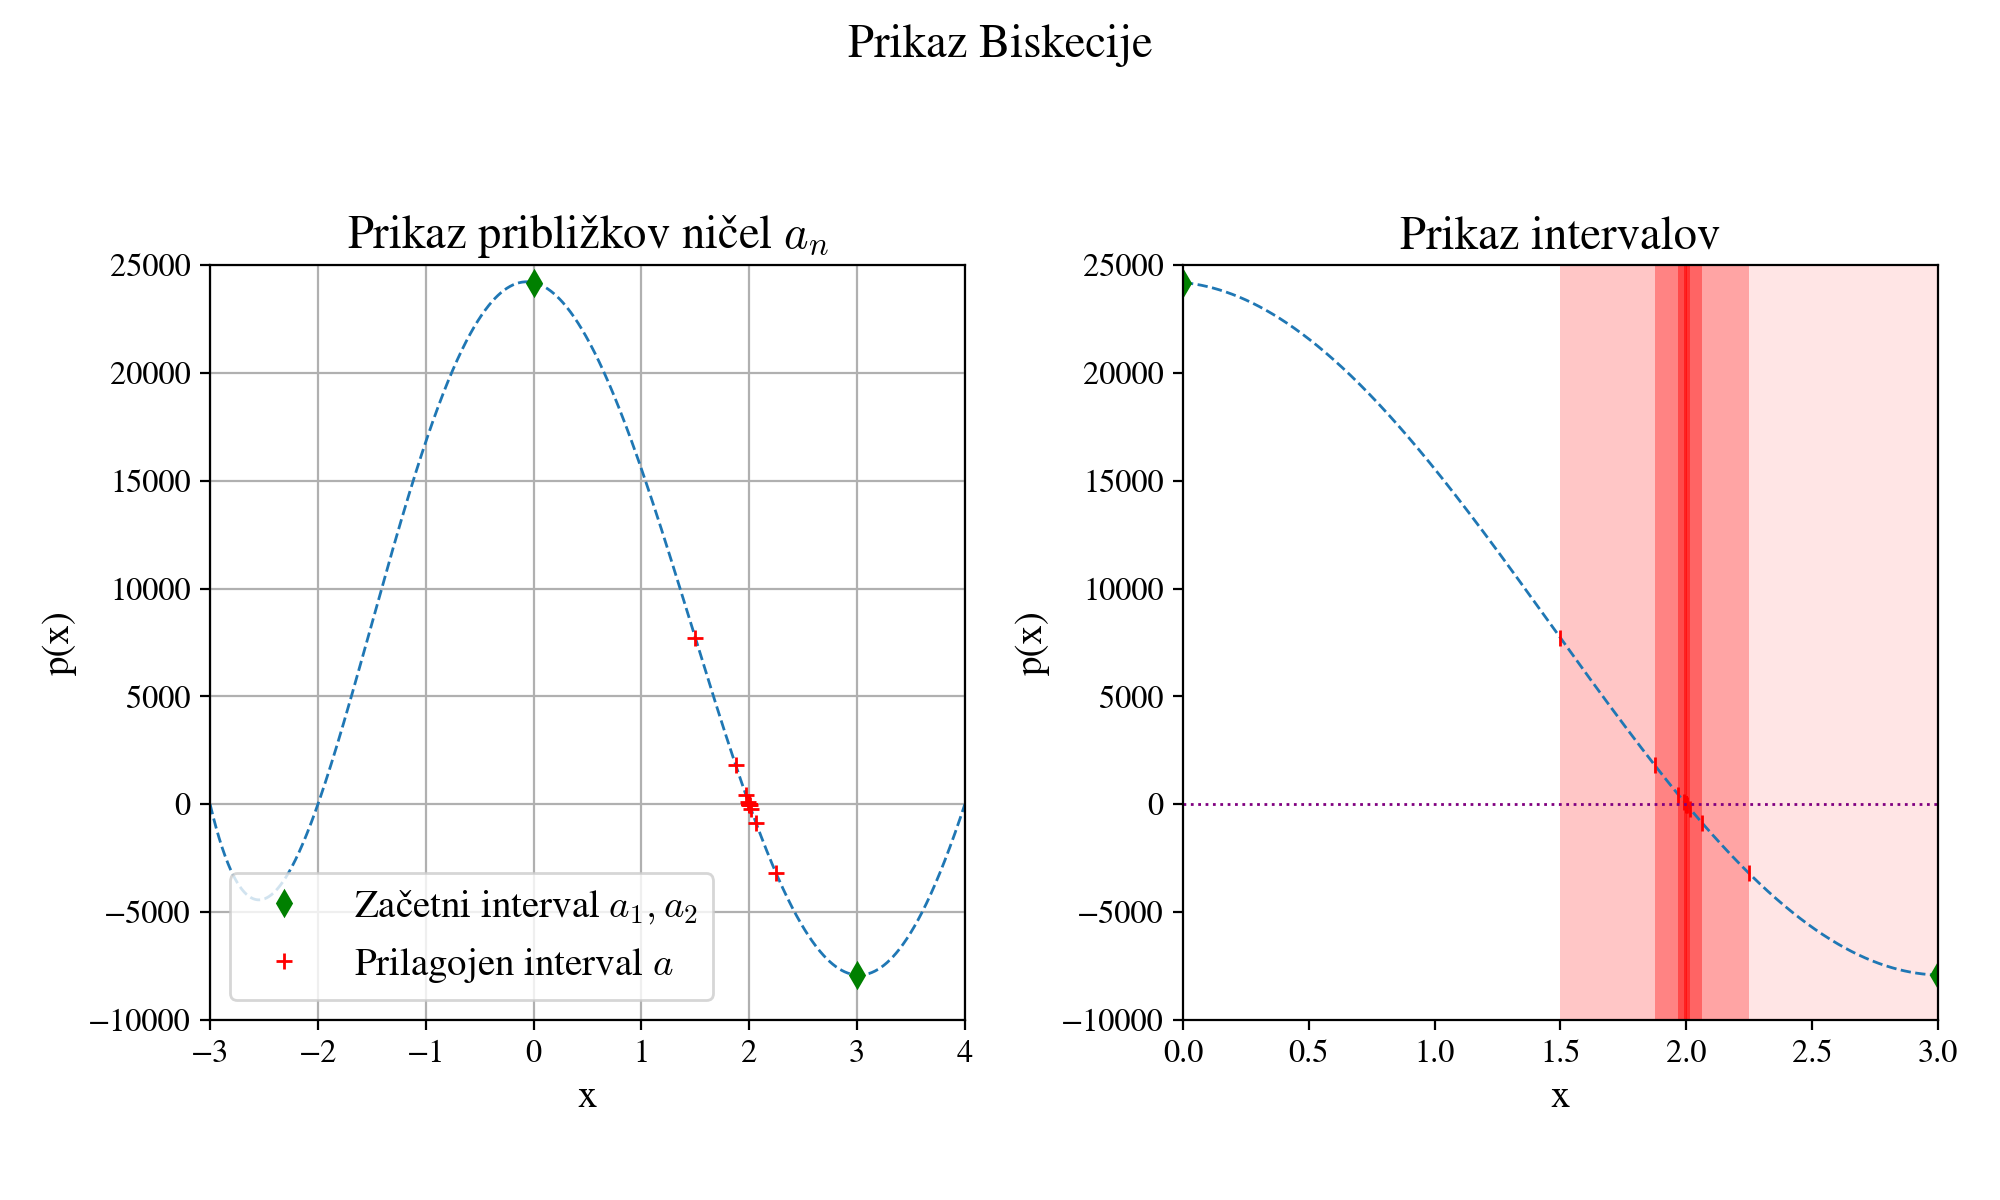
\includegraphics[width=1\textwidth]{img/bisection.png}
    \caption{Potek algoritma biskecije}
    \label{fig:bisection}
\end{figure}
\noindent
\textit{Hitro lahko opazimo, da bisekcija deluje kot opisano. Rdeči $+$ predstavljajo pridobljen $a$. Opazimo, da se ta razpolavljaj, tako da velikost interval konvergira proti 0. Seveda je za to potrebna tudi pravilna izbira prvotnega intervala}.
    
\end{primer}






\subsection{Newtonova metoda}
Najpogostejša in najbolj poznana metoda za iskanje ničel se imenuje Newtonova oz. tangentna metoda. Metoda je v resnici le poseben primer navadne iteracije. Navadna iteracija je preprosto metoda, kjer približek $x_r$ zapišemo v oblik $x_{r+1} = \mathcal{I}(x_r)$, $\mathcal{I}$ predstavlja iteracijsko funkcijo. Iteracijska funkcija mora izpolnjevati določene pogoje, ki so opisani v \cite{Plestenjak2010}. Tangenta metoda uporablja tangento, ki se dotika funkcije v toči $(x, p(x))$. Ničla tangente nato predstavlja približek ničle funkcije. Matematično gledano Newtonova metoda izhaja iz Taylorjevega izreka. Naj bo $x_r$ tangenti približek (oz. prvotni približek, če je iteracija prva) in $h$ zamik, ki ga opravimo v iteraciji. Funkcijo razvijemo v Taylorjevo vrsto:
\begin{align}
    f(x_r + h) = f(x_r) + \frac{f'(x_r)}{1!}h + \frac{f''(x_r)}{2!}h^2 + \mathcal{O}(h^3)
\end{align}
Zanemarimo višje člene vrste, tako da dobimo tangento (približek z linearno funkcijo). Ovrednotili bi radi ničlo tangente torej $ f(x_r + h) = 0$
\begin{align}
    f(x_r + h) \approx f(x_r) + f'(x_r)h  \xrightarrow[]{f(x_r + h) = 0} f(x_r) + f'(x_r)h \approx 0
\end{align}
Izpostavimo $h$, da dobimo nov zamik iteracije
\begin{align}
    h = -\frac{f(x_r)}{f'(x_r)}
\end{align}
Sedaj lahko zapišemo zamik v obliki algoritma naravne iteracije

\begin{align}
    x_{r+1} = \mathcal{I}(x_{r}) = x_{r} + h =  x_{r} - \frac{f(x_r)}{f'(x_r)}
\end{align}
Preprosto algoritem ovrednoti nov zamik iteracije glede na ničlo tangente prejšne iteracije.
\begin{algorithm}[H]
\caption{Newton-Raphsonova metoda}
\begin{algorithmic}



\Procedure{DiskretniOdvod}{$x, h$} \Comment{Najdi diskretni odvod $\Tilde{f'}(x)$}
    \State \Return $\frac{p(x + h) - p(x)}{h}$ \Comment{$h$ predstavlja natančnost diskretnega odvoda}
\EndProcedure\\
\Require $x_r$

\Procedure{NajdiNičlo}{}
\While{$|f(x_r)| > \epsilon$} \Comment{Iteriraj dokler ni $p(x_r)$, v okolici ničle}
    \State $d \gets f'(x_r)$ \Comment{Odvjaja diskretno ali analtično, če je možno}
    \State $x_r \gets x_r - \frac{f(x_r)}{d}$
\EndWhile 
\State  \Return $x_r$
\EndProcedure
\end{algorithmic}
\end{algorithm}
\newpage
\begin{primer}
    Najdi ničlo polinoma $p(x) = (x+3)(x+2)(x+8)(x+1)(x-2)(x-4)$
    \begin{figure}[H]
    \centering
    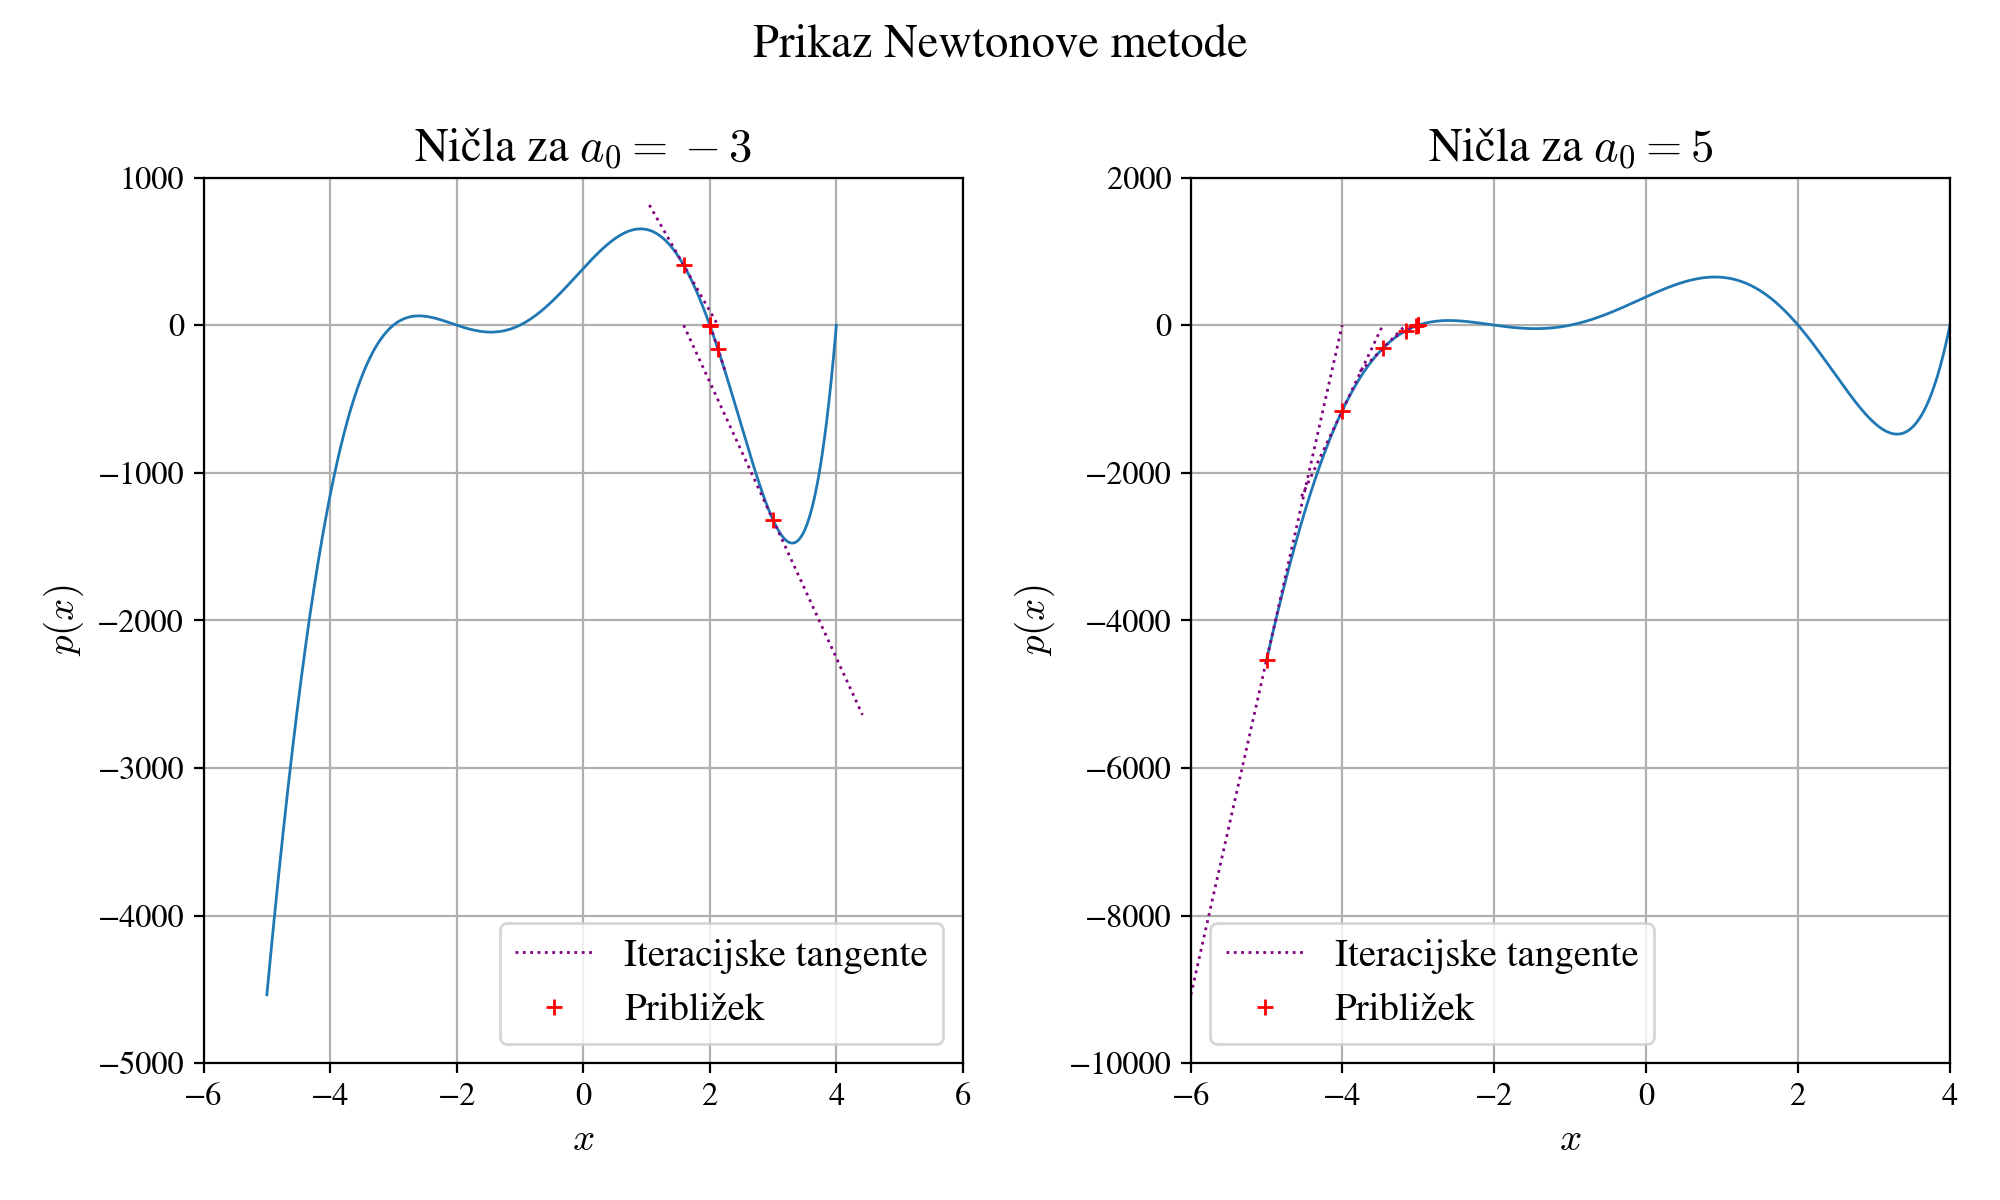
\includegraphics[width=1\textwidth]{img/newton.png}
    \caption{Potek algoritma Newtonove metode}
    \label{fig:newtons}
\end{figure}
    Za dva različna približka nam algoritem vrne najbližjo ničlo. Algoritem konvergira veliko hitreje kot bisekcija, obenem je  ničla tudi natančnejša, a več o tem kasneje. Opazimo lahko da se nov približek označen z rdečim + nahaja rano tam kjer tangenta seka ničlo, kar potrdi pravilno implementacijo metode.
\end{primer}
\section{Posebne metode}
Veliko smo že povedali o metodah za iskanje ničel, nič pa še nismo povedali o metodah iskanje več ničel polinoma. Iskanje več ničel, kot smo že omenili, predstavlja velike probleme. Večino iterativnih algoritmov je bolj ali manj neuporabnih, ker je konvergenca teh slaba v okolicah, kjer se ničla ne nahaja. Omenili smo eno od tehniki izločanja ničel, ampak kot smo že povedali je konvergenca tovrstnih metod slaba. Zato se ponavadi uporabljajo posebni algoritmi in metode, ki delajo le za iskanje ničel polinomov. Prva metoda je zelo preprosta obenem pa tudi (skoraj) vedno konvergira. Polinome zapišemo v obliki pridružene matrike (\textit{Companion matrix}) \cite{Plestenjak2010}. Za poljuben polinom $p(x)$, lahko z njegovimi koeficienti sestavimo sledečo matriko

\begin{align}
    C(p)={\begin{bmatrix}0&0&\dots &0&-a_{0}\\1&0&\dots &0&-a_{1}\\0&1&\dots &0&-a_{2}\\\vdots &\vdots &\ddots &\vdots &\vdots \\0&0&\dots &1&-a_{n-1}\end{bmatrix}}
\end{align}

$a_0, a_1, ... a_k \in \Vec{a}$ predstavljajo koeficiente polinoma. Obstaja več zapisov za pridruženo matriko. Zapis matrike (2) se uporablja najpogosteje. Ničle polinoma tovrstne matrike so lastne vrednosti matrike, torej
\begin{align}
    C(p) \Vec{x} = \lambda \Vec{x}
\end{align}
$\lambda$ predstavlja lastno vrednost. Problem iskanja ničel se torej spremeni v problem iskanja lastnih vrednosti. Seveda pa za polinome zelo visokega reda tovrstni algoritem ni primeren, ker velja, da je časovna kompleksnost algoritmov za iskanje lastnih vrednosti razpršenih matrik (matrik z veliko ničlami) enaka $\mathcal{O} (ck^2)$. $k$ v izrazu za kompleksnost predstavlja stopnjo polinoma, ter red matrike (matrika je reda $k\times k$).
\begin{primer}
    Matrika je v računalništvu le več dimenzionalni seznam. Razpršena matrika (na levi) je več dimnezionalni seznam, ki vsebuje veliko ničel, medtem ko gosta matrika (na desni) vsebuje predvsem ne ničelne elemente.

    \begin{align}
     \begin{bmatrix}
34 & 12 & 0 & 0 & 0 & 0 \\
0 & 7856 & 68 & 0 & 0 & 0  \\
0 & 0 & 456 & 54 & 0 & 0 \\
0 & 0 & 0 & 654 & 227 & 0 \\
0 & 0 & 0 & 0 & 45 & 23 \\
0 & 0 & 0 & 0 & 0 & 54 \\
\end{bmatrix}  
\qquad
         \begin{bmatrix}
34 & 12 & 32 & 1 & 32 & 43 \\
37 & 7856 & 68 & 76 & 4 & 2 \\
54 & 324 & 456 & 54 & 34 & 41 \\
65 & 34 & 456 & 654 & 227 & 675 \\
43 & 456 & 435 & 87 & 45 & 23 \\
23 & 45 & 234 & 34 & 21 & 54 \\
\end{bmatrix}  
    \end{align}
\end{primer}

Mi se ne bomo preveč osredotočali na algoritme za iskanje lastnih vrednost in preprosto uporabili algoritem, ki ga ponuja \texttt{scipy}. Zaradi konvergence in hitrost algoritma za manjše matrike se ta metoda velikokrat uporablja za ovrednotenje rezultatov brskanja na različnih brskalnikih (Google, Bing, ...), kot primarno metodo jo pa uporablja tudi \textit{Matlab}.

\begin{algorithm}[H]
\caption{Izračun večih ničel}
\begin{algorithmic}
\Require $p$
    \State $C \gets \Call{GenerateMatrix}{p}$ \Comment{Ustavri pridruženo matriko iz polinoma $p$}
    \State $D \gets \Call{DenseMatrix}{p}$ \Comment{Matriko \textbf{lahko} iz razpršene pretvorimo v gosto}
\Return \Call{FindEigenValues}{$C \lor D$} \Comment{Najdi lastne vrednosti matrike}
    
\end{algorithmic}
\end{algorithm}
Iskanje lastnih vrednosti matrike lahko opravimo na tako razpršenih kot gostih matrikah. Ponavadi moramo za iskanje \textbf{vseh lastnih vrednosti} uporabiti gosto matriko, ker je konvergenca algoritmov za razpršene matrike slabša. V primeru, da iščemo le nekaj lastnih vrednosti (oz. ničel) pa so algoritmi, kot so Laczosev in Arnoldijev algoritem za razpršene matrike seveda boljši \cite{Plestenjak2021}. Ko govorimo o pretvorbi iz razpršene v gosto matriko govorimo o načinu shranjevanja matrike na notranjem pomnilniku \textit{in ne o matematičnem pomenu tovrstnih matrik}. Razpršena matrika je na notranjem pomnilniku shranjena v obliki manjšega seznama (\textit{array}). Elementi sesznama so seznami oblike \texttt{\{int x, int y, double st\}}. Torej je v resnici ta seznam le $n \times 3$ matrika. V algoritmih, kjer nastopajo razpršene matrike, so tako vsi elementi pridružene matrike, ki niso v množici razpršene matrike opredeljeni z 0. To nam omogoča, da prihranimo na prostoru, ki ga matrika zasede na notranjem pomnilniku. Če uporabljamo goste matrike so pa v nasprotju s razpršenimi matrikami na notranjem pomnilniku zapisani tudi elementi s številom 0. Seveda za matrike, ki niso razpršene, razpršena matrika vzame več prostora na notranjem pomnilniku. Obenem pa so algoritmi, ki so definirani v razredih razpršenih matrik, namenjeni le razpršenim matrikam in zato so matematično hitrejši le v primeru, da so matrike res razpršene \cite{sparsem}. Nesemo pozabiti tudi, da so moderne centralne procesne enote optimizirane za množenje gostih matrika.
\begin{primer}
    Poišči vse ničle polnoma podanega s predpisom $p(x) = \sum_{n=0}^{24} (-1)^n \frac{x^{2n+1}}{(2n+1)!}$ s pomočjo pridružene matrike. Izvorna koda je v prilogi.
    \begin{figure}[H]
    \centering
    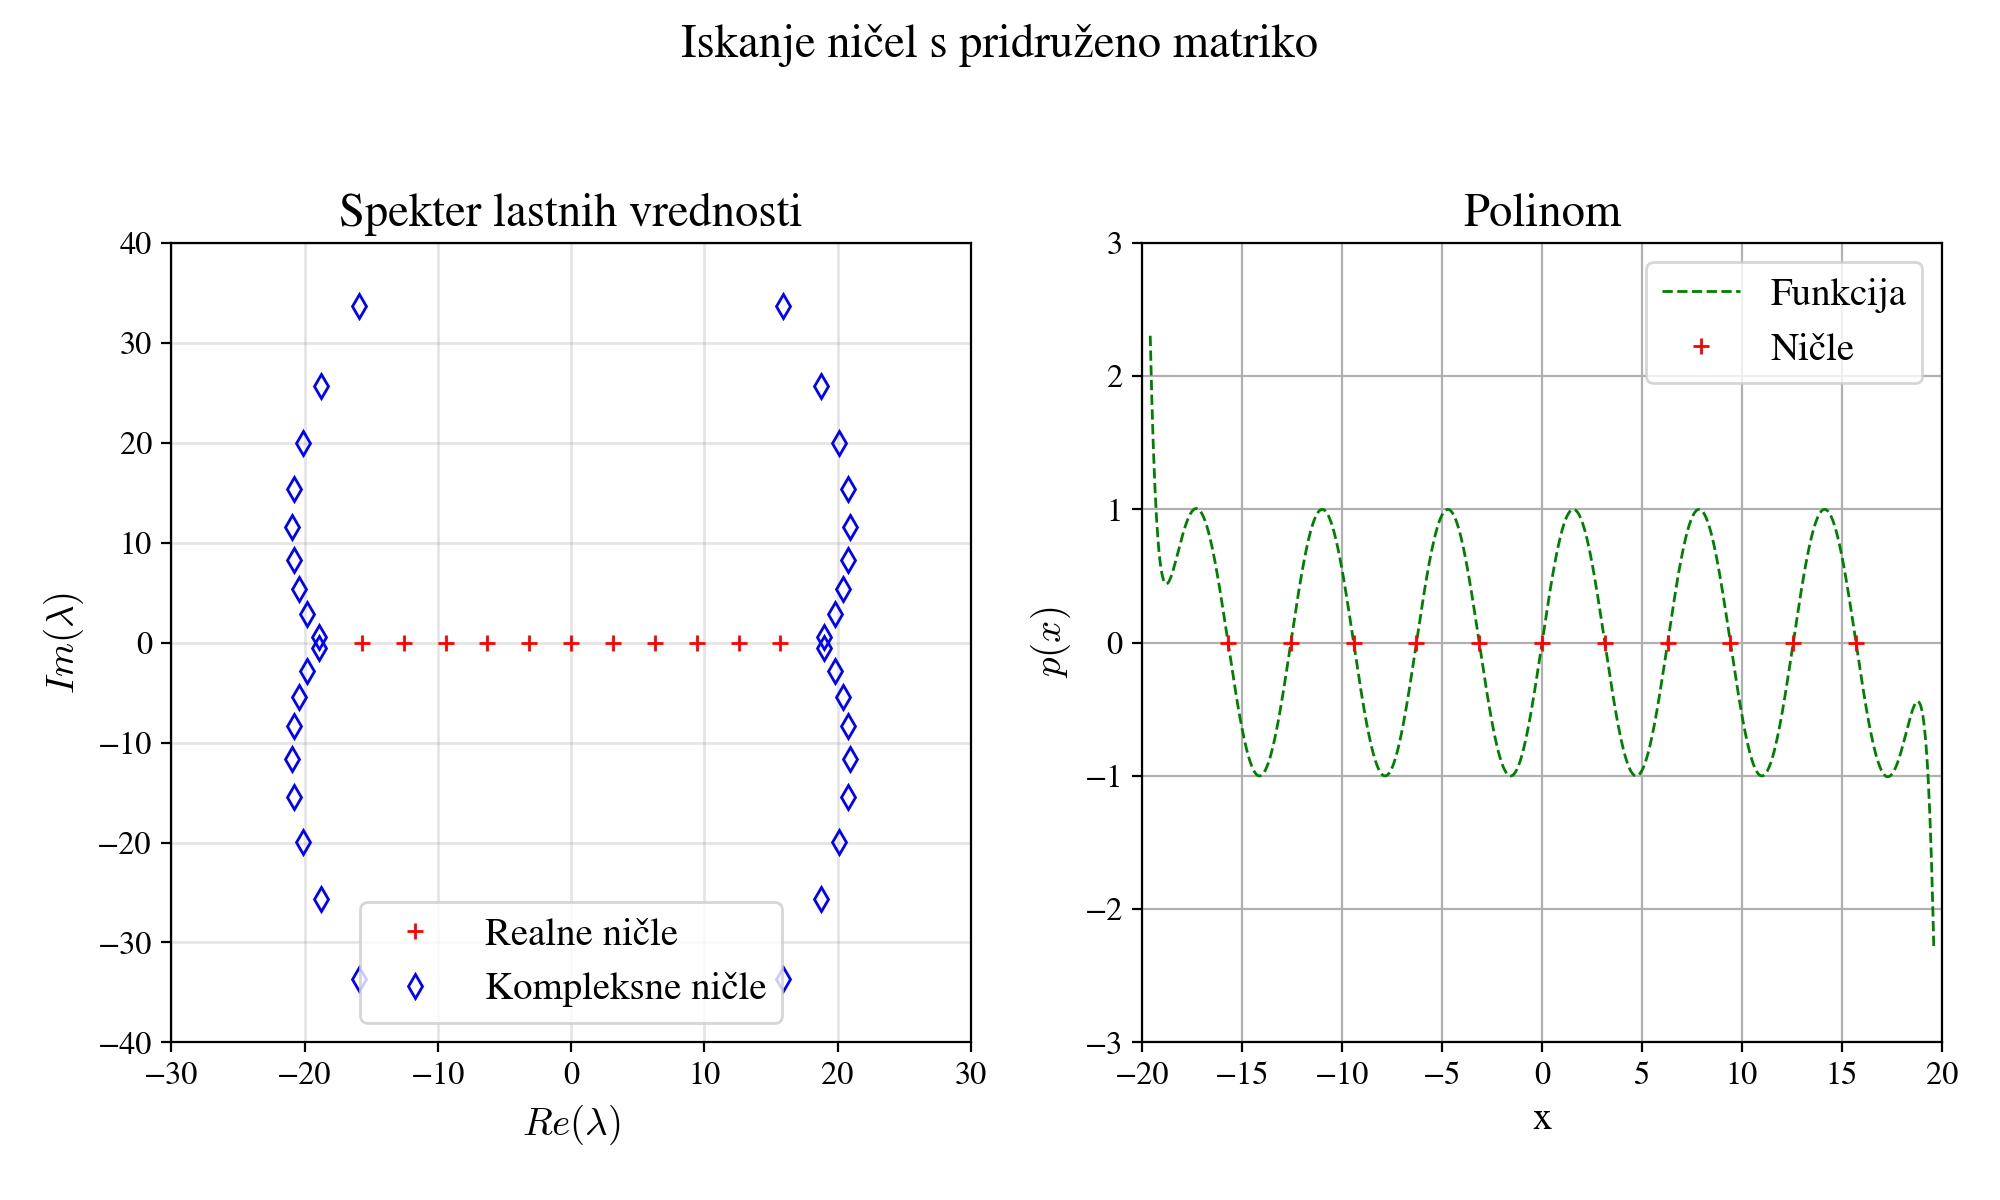
\includegraphics[width=1\textwidth]{img/eigenvalue.png}
    \caption{Potek algoritma s pridruženo matriko}
    \label{fig:companionmatrix}
\end{figure}
Opazimo lahko, da je vsaka lastna vrednost (Slika \ref{fig:companionmatrix}), ki ima le realni del na spektru, tudi ničla polinoma. To tudi potrjuje pravilnost našega algoritma. Za iskanje lastnih vrednosti smo uporabili kar funkcijo \texttt{eigs}, ki jo ponuja \texttt{numpy}. Matirka je sicer razpršena, zato bi bila hitrejša metoda verjetno \texttt{sparse.linalg.eigs}, ki jo ponuja \texttt{scipy}.
\end{primer}
Metoda pridružene matrike je sicer res iterativna, ker se lastne vrednosti ponavadi iščejo iterativno, vendar težko rečemo, da je direktno iterativna kot prejšne metode. Za polinome so bile razvite še druge posebne iterativne metode za iskanje več ničel. Metode konvergirajo veliko hitreje, kot metoda pridružene matrike. Obenem pa konvergirajo za (skoraj) vsak začetni približek. Mi se bomo osredotočili predvsem na dve metodi Laguerreovo in Durand-Kernejevo. Obstaja še veliko metod, tudi nekaj novejši, ki so v nekaterih primerih hitrejše.
\subsection{Laguerreova metoda}
Laguerreova metoda je najpreprostejša metoda za izračun ničel polinomov. Za polno izpeljavo bi potrebovali nekaj matematičnih dokazov o občutljivosti ničel, ki jih ne bomo opisali. Izreki in moderna modificirana implementacija so opisani v \cite{lagguerrmetoda}. Če zapišemo polinom v faktorizacijski obliki dobimo $p(x) = \alpha_k (x - x_1)(x - x_2)...(x - x_n)$. Definiramo dve vsoti vrst (izpeljani v \cite{Plestenjak2010}):
\begin{align}
    S_1(x) &= \sum_{i=1}^n \frac{1}{x-x_i} = \frac{p'(x)}{p(x)}\\
    S_2(x) &= \sum_{i=1}^n \frac{1}{(x-x_i)^2} = -S_1'(x) = \frac{p'^2(x) - p(x)p''(x)}{p^2(x)}
\end{align}
S pomočjo manipulacije teh vrst \cite{Plestenjak2010} lahko nato izrazimo iteracijsko funkcijo $\mathcal{I}$.
\begin{align}
    x_{r+1} = x_r - \frac{n}{S_1 \pm \sqrt{(n-1)(nS_2-S_1^2)}}
\end{align}
Zaporednje $x_{r+1}$ nam vrne približke ničle polinoma. Obstaja zelo malo primerov, kjer ta metoda konvergira počasi zato je pogosto uporabljena kot primerna metoda za izračun ničle polinomov višjega reda. Za izračun več ničel s tovrstno metodo je potrebno spreminjat začetni približek $x_0$. Prednost te metode je, da za razliko od Newtonove metode, ta metoda hitreje konvergira proti ničli, in da najde skoraj vse ničle, četudi so te skupaj (to je pogojeno z natančnostjo plavajočih vejic, če so ničle preveč skupaj jih ne moramo razlikovati).

\begin{algorithm}[H]
\caption{Laguerreova Metoda}
\begin{algorithmic}

\Procedure{NajdiNičlo}{$x_r$}
\While{$|f(x_r)| > \epsilon$} \Comment{Iteriraj dokler ni $p(x_r)$, v okolici ničle}
    \State $d \gets f'(x_r)$ \Comment{Odvjaja diskretno ali analtično, če je možno}
    \State $d_2 \gets f'(f'(x_r))$
    \State $S_1 \gets \frac{d}{f(x_r)}$
    \State $S_2 \gets \frac{d^2 - f(x_r)d_2}{f^2(x_r)}$
    \State $x_r \gets x_r - \frac{n}{S_1 \pm \sqrt{(n-1)(nS_2-S_1^2)}}$
\EndWhile 
\State  \Return $x_r$
\EndProcedure
\\
\Procedure{VečNičel}{$i_{max}, x_z, h$}
\State $\mathbb{S} \gets \{\}$
\While{$k \le n$} \Comment{Iteriraj doklar ni število ničel enako stopnji polinoma}
    \If{$i > i_{max}$} \Comment{Meja iteraciji, če algoritem ne konvergira}
        \State \Return $\mathbb{S}$
    \EndIf
    \State $x_r \gets x_r \pm h$ \Comment{Nov začetnik približek}
    \State $i \gets i + 1$ 
    \State $x \gets \Call{NajdiNičlo}{x_r}$
    \If{$x \not\in \mathbb{S}$} \Comment{Poglej če je ničla že v množici ničel}
    \State $\mathbb{S} + \{x\}$ 
    \EndIf
\EndWhile 
\EndProcedure\\

\end{algorithmic}
\end{algorithm}
\newpage
\subsection{Durand–Kernerjeva metoda}
Zadnja metoda, ki jo bomo opisali je Durdand-Kernerjeva metoda. Metoda je samo po sebi dokaj komplicirana, cel matematičen postopek je opisan v \cite{Bohte_1993}. Mi bomo metodo opisal preprosto. Za polinom $p(x) = \alpha_k (x-x_1)(x-x_2)...(x-x_k)$ iščemo popravek oz. približek $\Delta x_i$. Torej
\begin{align}
    p(x) = (x-(x_1 + \Delta x_1))(x-(x_2 + \Delta x_2))...(x-(x_k + \Delta x_k)) 
\end{align}
Iz izraza izpostavimo približek $\Delta x$ in zanemarimo višje člene (postopek je opisan v \cite{Bohte_1993, Plestenjak2010}). Iz izraza lahko sedaj izpostavimo $\Delta x_n$ in dobimo.
\begin{equation}
    \Delta x_n = \frac{-p(x_n)}{\displaystyle \prod_{i=1, i \ne n}^k (x_n - x_i)} \Bigg \rbrace \quad \text{\textit{$n$ predstavlja eno izmed ničlo}}
\end{equation}
Sedaj lahko to zapišemo v obliki iteracijske funkcije $\mathcal{I}$
\begin{align}
    x_i^{r+1} = x_i^r - \Delta x_i(x_r).
\end{align}


Dobimo preprosto iteracijo za izračun vseh ničel. Tovrstni algoritem nam omogoča, da imamo za vsako ničlo posebej prvotni približek, ki nato konvergira proti vsaki ničli posebej. Potemtakem ne potrebujemo več pregledovati pogoja če je ničla že v množici (seznamu) ničel. 
Upoštevati moramo, da morajo biti začetni $x_r$ paroma različni sicer algoritem divergira, ker se v imenovalcu izraza za $\Delta x_n$ pojavi nič. Obstajajo tudi druge izepljave algoritmov, ki omogočajo bolj stabilna konvergenco. Opazili bomo, da nekatere ničle metode za slabe začetne približke hitro divergirajo.



\begin{algorithm}[H]
    \caption{Durand–Kernerjeva metoda}
    \begin{algorithmic}
    \Require $k, n_{max},  \Vec{x}^1$ \Comment{Red polinoma, maksimalno št. iteraciji in prvotni približek}
    \While{ $n < n_{max}$}
    \For{ $i \gets 1$ to $k$ } \Comment Iteriraj skozi vse ničle
        \If{$|p(x_i^n)| \le \epsilon$}  \Comment{Iteriraj dokler ni $p(x_r)$, v okolici ničle}
            \State \Return $x_i^n$
        \EndIf
        \State $p = 1$ \Comment{Pripravi $p$ za izračun produkta  $\prod_{i=1, i \ne n}^k (x_n - x_i)$}
        \For{$h \gets 1$ to $k$}
            \If{ $h \ne i$}
                \State $p \gets p \cdot (x_i^n - x_h^n)$
            \EndIf
        \EndFor
        \State $\Delta x_i \gets \frac{f(x_i)}{p}$
        \State $x^{n+1}_i = x^n_i - \Delta x_i$
    \EndFor
    \EndWhile
    \end{algorithmic}
    \end{algorithm}
    Kot že omenjeno obstajajo tudi druge izpeljave. Najbolj poznana formulacija je definitivno kvadratna implementacija. V imenovalcu te metode zapišem
    \begin{equation}
        \Delta x^{r+1}_n = \frac{-p(x_n)}{\displaystyle \prod_{i=1}^{n-1} (x^r_{n} - x^{r+1}_i)  \prod_{i=n+1}^{k} (x^r_n - x^r_i)} 
    \end{equation}
    Tovrstna izpeljava izboljša konvergenco. Mi se bomo sicer držali originalne implementacije, ker ima kvadratna metoda svoje probleme. Problemi se izražajo predvsem v obliki hitrih divergence ničel z slabim začetnim približkom.
    \newpage
\begin{primer}
    Poišči vse ničle polinoma poljubnega polinoma s Durand Kernerjevo metodo. Izvorna koda je v prilogi.
    \begin{figure}[H]
    \centering
    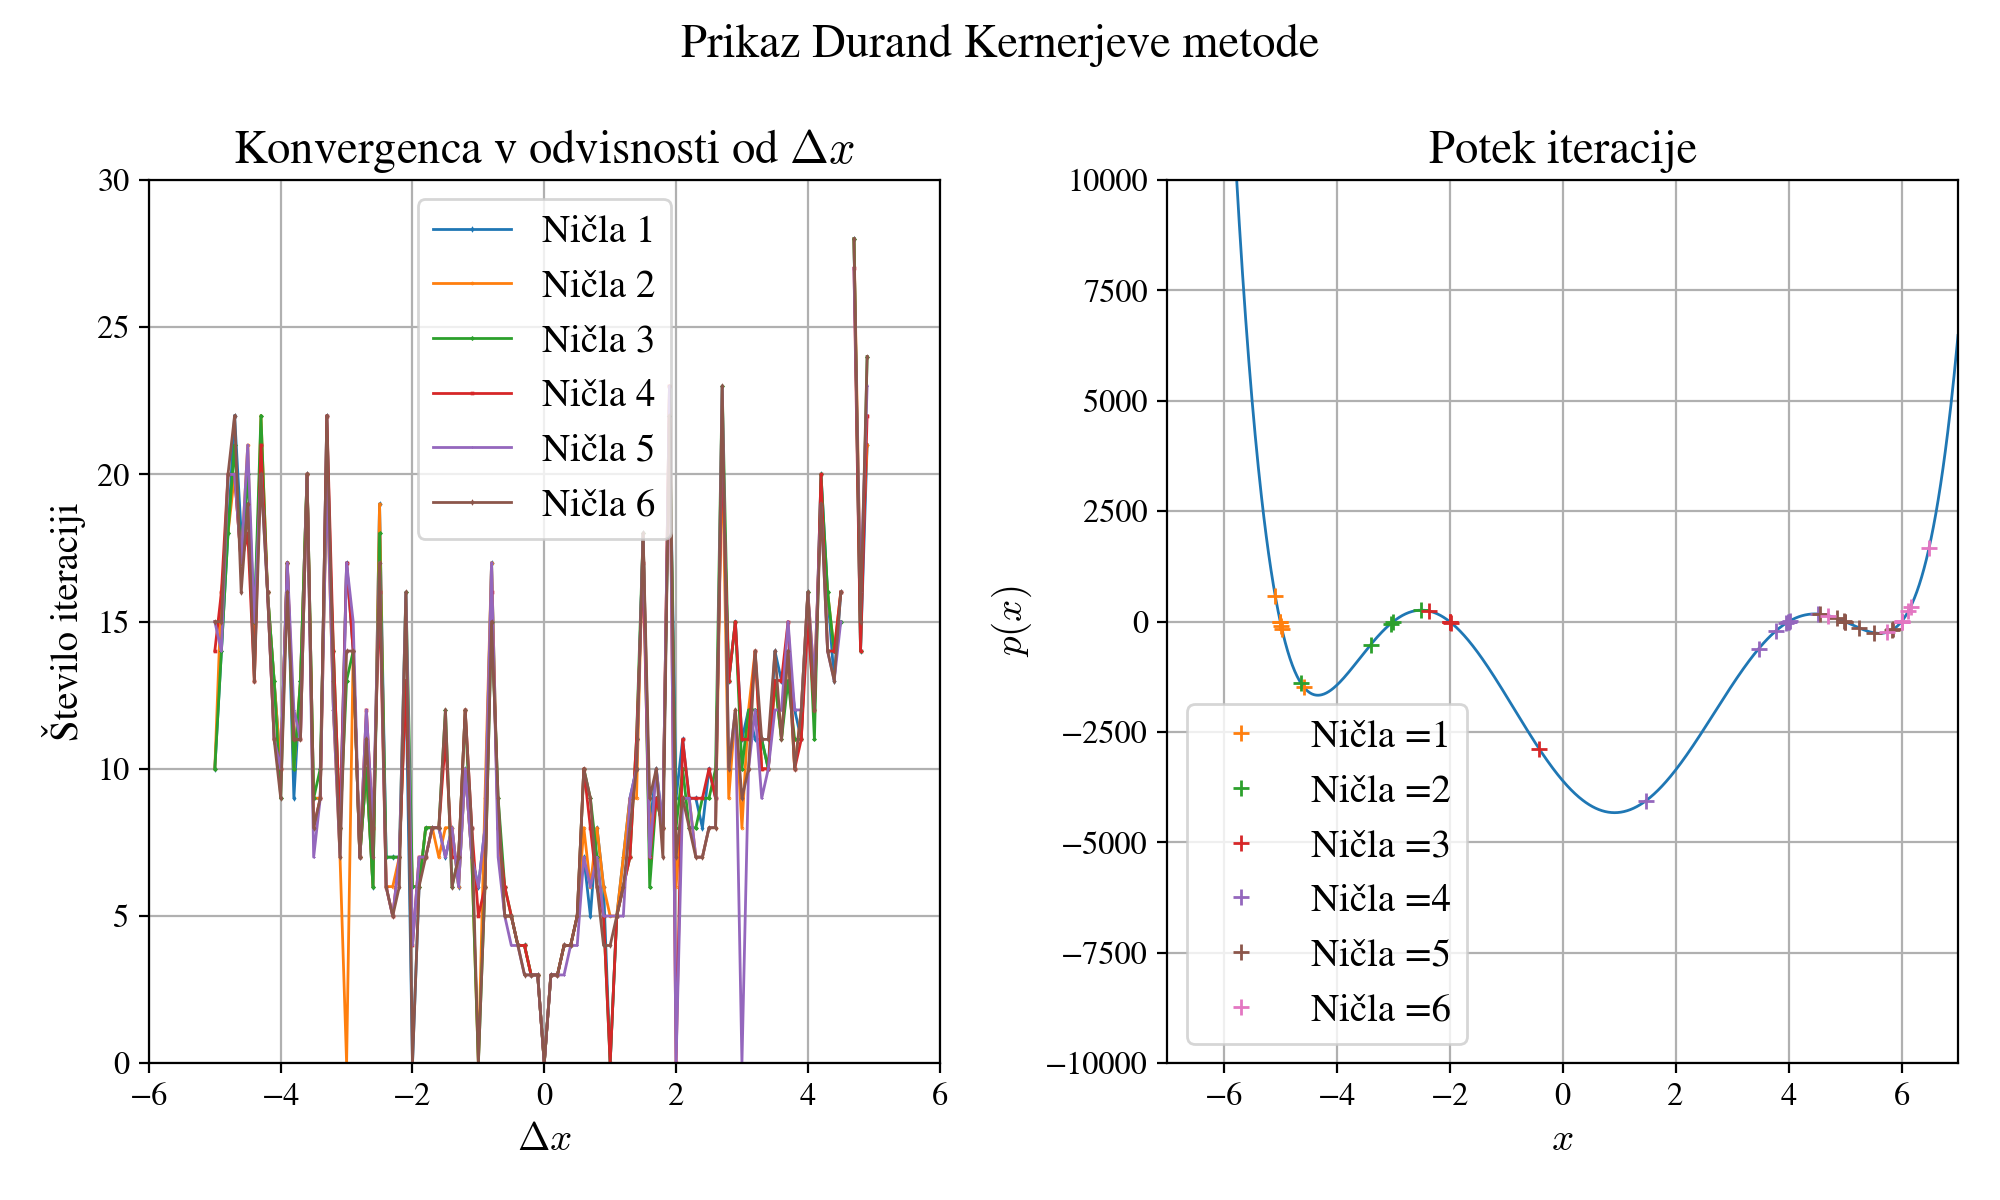
\includegraphics[width=1\textwidth]{img/durand.png}
    \caption{Potek Durand-Kernerjevega algoritma}
    \label{fig:durand}
\end{figure}
$\Delta x$ predstavlja razdaljo od ničle do prvotnega približka. Opazimo, da metoda deluje. Pričakovano potrebuje metoda več iteraciji glede na oddaljenost prvotnega približka od ničle. Zanimivo je mogoče dejstvo, da če so prvotni približki preveč skupaj algoritem zelo hitro divergira. Obenem hitro divergira tudi če prvotni približki niso dobro sortirani. Več o sami konvergenci bomo povedali v 4. poglavju.
\end{primer}


\newpage
\chapter{Algoritmi v $\R^n$}
Do sedaj smo omenili le algoritme, ki iščejo ničle funkciji z 1 spremenljivko. Pogosteje pa se znajdemo pri problemih funkciji, ki so odvisne od več spremenljivk. Algoritmi za iskanje ničel funkciji več spremenljiv so še posebej pomembni v optimizacijskih problemih, kjer moram ponavadi minimizirat funkcijo na katero vpliva več faktorjev. Naj bo $p: \R^n \to \R$ polinom. Predpis polinoma je
\begin{align}
    p(x_1, x_2, x_3, ..., x_n) = \sum_{h = 0}^{x_1_{s}} \alpha_{1,h} x_1^h + \sum_{h = 0}^{x_2_{s}} \alpha_{2,h} x_2^h + ... + \sum_{h = 0}^{x_n_{s}} \alpha_{n,h} x_n^h = \sum_{\ell = 1}^n\sum_{h=0}^{x_{\ell}_s} \alpha_{\ell, h} x_\ell^h
\end{align}

Obstaja le peščica algoritmov, ki lahko izračunajo ničle tovrstnih funkciji. Računalniško gledano se največkrat uporablja posplošitev bisekcije. Namesto na interval se sedaj osredotočamo na regijo v prostoru. Algoritma je le posplošitev že izpeljanega algoritma, zato ga ne bomo izpeljali še enkrat. Namesto mej intervala sedaj izberemo mejne točke, ki predstavljajo regijo, tako da ima na mejnih točka funkcija nasprotna si predznaka, nato regijo manjšamo po vseh prostorskih spremenljivkah. Obstaja tudi algoritem, ki je posledica Poincare-Mirandovega izreka \cite{Kulpa1997}, vendar je algoritem zapleten.

V optimizacijskih problemih se več ne išče ničel funkcije odvoda, temveč operatorjev, ki delujejo na funkcijo. Najbolj znana je Newtonov algoritem konjugiranega gradianta, ki ga bomo kot edinega predstavili. Obstajajo pa seveda bolj kompleksni algoritmi kot so konjugirana vektorska metoda, Broyden–Fletcher–Goldfarb–Shanno algoritem,Nelder-Mead simpleks,... 

\subsection{Newtonova metoda konjugiranega gradienta}
Za poljubno funkcijo $f: \R^n \to \R$ velja, da jo lahko zapišem z Taylorjevo vrsto, kot kvadratno aproksimacijo
\begin{align}
    f(\Vec{x} - \Vec{a}) \approx f(\Vec{a})  + (Jf)(a)(\Vec{x} - \Vec{a}) +  \frac{1}{2} (\Vec{x} - \Vec{a})^T (Hf)(\Vec{a}) (\Vec{x} - \Vec{a})
\end{align}
$H$ predstavlja Hesejevo matriko (matriko drugih parcialnih odvodov), $J$ predstavlja Jacobijevo matriko (matriko prvih parcialnih odvodov). Jacobijeva matrika je v primeru skalarnega polja torej $\R^n \to \R$, le gradient. Gradient $\nabla f$ je preprosto vektor, ki kaže proti spremembi funkcije. Mi želimo izvedeti, kje ta funkcija doseže minimum, torej $\nabla f = 0$. Iz zgornje enačbe preprosto izrazimo $(Jf)(a)(x-a)$.
\begin{align}
    (Jf)(a)(\Vec{x} - \Vec{a}) = f(\Vec{x} - \Vec{a}) - f(\Vec{a}) - \frac{1}{2} (\Vec{x} - \Vec{a})^T (Hf)(\Vec{a}) (\Vec{x} - \Vec{a})
\end{align}
Sedaj primerjamo to z 0, da dobimo lokalni minimum (naj bo zamik $a=\Vec{0}$)
\begin{align}
    f(\Vec{x} - \Vec{a}) - f(\Vec{a}) - \frac{1}{2} (\Vec{x} - \Vec{a})^T (Hf)(\Vec{a}) (\Vec{x} - \Vec{a}) = 0 \xrightarrow{izepljava} (Hf)(\vec{x}) = -f(\vec{x})\  
\end{align}
$(Hf)(\vec{x}) = -f(\vec{x})$ je sedaj linearni problem, ki ga rešimo z algoritmom za reševanje sistema linearnih enačb.
\textbf{Ta metoda je izredno pomembna v strojnem učenju!}
\newpage
\chapter{Primerjava algoritmov in rezultati}
\todo[inline]{Tukaj pridejo različne primerjave konvergence in časovne zahtevnosti algoritmov. Konvergenčni test bo vključeval oddaljenost od ničle, povprečno napako glede na iteracijo ter št. iteraciji v odvisnosti od stopnje polinoma pri konstantnem $\Delta x$. Časovno zahtevnost bomo merili v odvisnosti od $\Delta x$ ter stopnje polinoma}
\section{Problemi v informatiki in računalništvu}
\todo[color=purple, inline]{Obravnavali bomo sledeče probleme. 
\begin{enumerate}
    \item Najnižja cena goriva (računalniše finance)
    \item 2 naključna optimizacijska primera, eden v odvisnosti od več spremenljivk spravi $\R^2$
    \item Optimizacijska naloga iz strojnega učenja in/ali kompresije podatkov
\end{enumerate}}
\newpage
\chapter{Zaključek}

\newpage
\noindent
\large \textbf{Zahvala} \\\\
\small
Zahvaljujem se mentorju mag. Tomi Zebiču za pomoč in nasvete pri pisanju seminarske naloge.
\newpage
\bibliography{literatura}
\bibliographystyle{acm}
\newpage
\appendix

\chapter{Algoritmi}
\section{Bisekcija}
\begin{mintedbox}{python}
polynomial = np.poly1d([4/9, 16, -1/2, 411/10, 3/2, 0, 7, 0, 2]) #ustvari polinom

def bisection(interval, eps):
    a = (interval[0] + interval[1]) / 2
    while abs(polynomial(a)) < eps:
        a = (interval[0] + interval[1]) / 2
        
        if(polynomial(a) * polynomial(interval[0]) < 0):
            interval[1] = a
        else:
            interval[0] = a
    return a

\end{mintedbox}

\section{Newtonov algoritem}

\begin{mintedbox}{python}
polynomial_coeffcient = np.polynomial.polynomial.polyfromroots([-3,-8,-2,-1,2,4])


polynomial = np.poly1d(np.flip(polynomial_coeffcient)) #ustvari polinom
polynomial_odvod = np.polyder(polynomial) #analitičen odvod polinoma

def newton(xr, eps):
    while abs(polynomial(xr)) > eps:
        xr = xr - polynomial(xr) / polynomial_odvod(xr)
    return xr
\end{mintedbox}
\section*{Algoritem pridružene matrike}

\begin{mintedbox}{python}
polynomial_coeffcient = np.polynomial.polynomial.polyfromroots([-3,-8,-2,-1,2,4])

companion_matrix = np.polynomial.polynomial.polycompanion(polynomial_coeffcient) #ustavri matriko (potrebuje ravno obraten red koeficientov)
polynomial_coeffcient.reverse()

polynomial = np.poly1d(polynomial_coeffcient) #ustvari polinom


eval, evec = np.linalg.eig(companion_matrix) #poišči ničle, prvi seznam lastne vrednosti drugi lastni vekotrji
\end{mintedbox}

\section{Laguerreov algoritem}

\begin{mintedbox}{python}
    polynomial_coeffcient = np.polynomial.polynomial.polyfromroots([-3,-8,-2,-1,2,4])


polynomial = np.poly1d(np.flip(polynomial_coeffcient)) #ustvari polinom
polynomial_odvod = np.polyder(polynomial) #analitičen odvod polinoma
polynomial_odvod_2 = np.polyder(polynomial, 2)



def laguerre(xr, eps):
    while abs(polynomial(xr)) > eps:

        s1 =  polynomial_odvod(xr)/polynomial(xr)
        s2 = (polynomial_odvod(xr)**2 - polynomial(xr) * polynomial_odvod_2(xr))/(polynomial(xr)**2)
        n = len(polynomial_coeffcient)

        xr = xr - (n) / (s1 - np.sqrt((n-1)*(n*s2-s1**2)))

    return xr
\end{mintedbox}

\section{Durand Kernerjev algoritem}

\begin{mintedbox}{python}
    polynomial_coeffcient = np.polynomial.polynomial.polyfromroots([-3,-8,-2,-1,2,4])


polynomial = np.poly1d(np.flip(polynomial_coeffcient)) #ustvari polinom


def durand(eps, approx):

    for n in range(0, 30):
        approx_cop = approx.copy()
        for i, x in enumerate(approx):
            if abs(polynomial(x)) < eps: 
                if(itearations_ap[i] == None):
                    itearations_ap[i] = n
                continue

            d = 1

            for k in approx_cop:
                if(k != x):
                    d = d * (x - k)

            approx[i] = x - (polynomial(x))/d
\end{mintedbox}
\end{document}
